\documentclass[conference]{IEEEtran}
\IEEEoverridecommandlockouts
% The preceding line is only needed to identify funding in the first footnote. If that is unneeded, please comment it out.
\usepackage{cite}
\usepackage{amsmath,amssymb,amsfonts}
%\usepackage{algorithmic}
\usepackage{graphicx}
\usepackage{float}
\usepackage{textcomp}
\usepackage{multirow}
\usepackage{subcaption}
\usepackage{xcolor}
\def\BibTeX{{\rm B\kern-.05em{\sc i\kern-.025em b}\kern-.08em
    T\kern-.1667em\lower.7ex\hbox{E}\kern-.125emX}}

\usepackage{tikz}
\usepackage{pgfplots}

\usepackage{algorithm}
\usepackage[noend]{algpseudocode}
\makeatletter
\renewcommand{\ALG@beginalgorithmic}{\footnotesize}
\makeatother

\algnewcommand\algorithmicswitch{\textbf{switch}}
\algnewcommand\algorithmiccase{\textbf{case}}
\algnewcommand\algorithmicotherwise{\textbf{otherwise}}

\algdef{SE}[SWITCH]{Switch}{EndSwitch}[1]{\algorithmicswitch\ #1\ \algorithmicdo}{\algorithmicend\ \algorithmicswitch}%
\algdef{SE}[CASE]{Case}{EndCase}[1]{\algorithmiccase\ #1}{\algorithmicend\ \algorithmiccase}%
\algdef{SE}[OTHERWISE]{Otherwise}{EndOtherwise}[1]{\algorithmicotherwise\ #1}{\algorithmicend\ \algorithmicotherwise}%
\algtext*{EndSwitch}%
\algtext*{EndCase}%
\algtext*{EndOtherwise}%

\usepackage[bahasa]{babel}

\begin{document}

\title{STUDI PERMASALAHAN \textit{K-MOST PROMISING PRODUCTS} BERBASIS INTERVAL WAKTU PADA DATA MULTIDIMENSI DENGAN SERIAL WAKTU}
\author{Hafara Firdausi, Bagus Jati Santoso, Henning Titi Ciptaningtyas\\
Departemen Informatika, Fakultas Teknologi Informasi dan Komunikasi, Institut Teknologi Sepuluh Nopember (ITS)\\
Jl. Arief Rahman Hakim, Surabaya 60111 Indonesia\\
\textit{e-mail}: hafarafirdausi@gmail.com\textsuperscript{1)}, bagus@if.its.ac.id\textsuperscript{2)}, henning@if.its.ac.id\textsuperscript{3)}
}

\maketitle

\renewcommand\abstractname{\textit{Abstrak}}
\renewcommand\IEEEkeywordsname{Kata kunci}

\begin{abstract}
Kemajuan ilmu pengetahuan dan teknologi telah mempengaruhi cara perusahaan dalam menjalankan bisnis, yaitu dengan mengumpulkan data preferensi pelanggan dari data penjualan produk, kemudian memanfaatkannya untuk mendapatkan informasi yang dapat digunakan untuk membuat keputusan bisnis yang tepat. Saat ini, sudah ada strategi pemilihan produk dengan melakukan pencarian $k$-produk yang paling banyak diminati oleh pelanggan, yaitu \textit{k-Most Promising Products (k-MPP)}. Sayangnya, komputasi k-MPP tidak mempertimbangkan variabel waktu dalam algoritme perhitungannya dan tidak dapat digunakan untuk memproses kueri berbasis interval waktu.

Artikel ini mengusulkan algoritme k-MPPTI \textit{(k-Most Promising Products in Time Intervals)} untuk menjawab permasalahan k-MPP berbasis interval waktu pada data multidimensi dengan serial waktu. Ada tiga jenis algoritme yang dibuat dan dibandingkan, yaitu k-MPPTI (menggunakan dua tipe kueri \textit{skyline}, yaitu \textit{dynamic skyline} dan \textit{reverse skyline}), k-MPPTI NoRSL (menggunakan kueri \textit{dynamic skyline} saja), dan k-MPPTI paralel (menggunakan teknik komputasi paralel). Efektivitas dan efisiensi algoritme diuji menggunakan data asli dan sintetis. Hasil uji coba menunjukkan bahwa algoritme k-MPPTI NoRSL dapat memberikan hasil dengan waktu eksekusi lima kali lebih cepat dan penggunaan memori satu kali lebih hemat dibandingkan dengan algoritme k-MPPTI.
\end{abstract}

\begin{IEEEkeywords}
Strategi pemilihan produk, Kueri, \textit{Dynamic skyline}, \textit{Reverse skyline}, Interval waktu
\end{IEEEkeywords}

\section{Pendahuluan}
Pesatnya kemajuan ilmu pengetahuan dan teknologi telah mempengaruhi cara perusahaan dalam menjalankan bisnis, yaitu dengan mengumpulkan data preferensi pelanggan dari data penjualan produk, kemudian memanfaatkannya secara cerdas untuk mendapatkan informasi yang dapat digunakan untuk membuat keputusan bisnis yang tepat. Misalnya, dengan mendapatkan informasi $k$-produk yang paling diminati oleh pelanggan beserta fitur-fiturnya, perusahaan dapat menentukan harga produk baru yang akan diluncurkan atau menentukan fitur apa yang diunggulkan dari produk baru yang hendak diproduksi. 

Saat ini, sudah ada penelitian yang mengembangkan strategi pemilihan produk dengan melakukan pencarian $k$-produk yang paling banyak diminati oleh pelanggan. Islam dan Liu (2010) memodelkannya sebagai kueri \textit{k-Most Promising Products} (k-MPP) \cite{kmpp} serta membuat kerangka kerja algoritme untuk memproses kueri tersebut. Komputasi k-MPP menggunakan dua tipe kueri \textit{skyline}, yaitu \textit{dynamic skyline} \cite{dynamic-skyline} dan \textit{reverse skyline} \cite{reverse-skyline}. Kueri \textit{dynamic skyline} digunakan untuk mengambil data produk terbaik berdasarkan sudut pandang pelanggan, sedangkan kueri \textit{reverse skyline} digunakan untuk mengambil data pelanggan potensial berdasarkan sudut pandang produk atau perusahaan \cite{kmpp}.

Sayangnya, komputasi k-MPP tidak mempertimbangkan variabel waktu dalam algoritme perhitungannya sehingga informasi yang didapatkan kurang valid dengan kondisi yang sebenarnya. Komputasi k-MPP juga tidak dapat memproses kueri berbasis interval waktu. Sebagai contoh, pertanyaan yang mungkin diajukan adalah \textit{"$k$-produk apa yang paling banyak diminati oleh pelanggan pada bulan Februari hingga September?"}. Dalam hal ini, bulan Februari hingga September disebut dengan interval waktu kueri dan data yang berbasis interval waktu disebut dengan data \textit{time series} atau serial waktu.

Sebagai ilustrasi, produk A adalah produk yang paling banyak diminati oleh pelanggan pada bulan Januari hingga Juni, namun posisinya diungguli oleh produk B yang lebih diminati pelanggan pada bulan Juli hingga September. Pada bulan Oktober, produk B tidak diproduksi lagi karena suatu alasan, sehingga produk A kembali diminati pelanggan. 

Berdasarkan ilustrasi tersebut, produk yang paling unggul berdasarkan kueri k-MPP adalah produk B karena produk B pernah mengungguli produk A walaupun rentang waktu unggulnya lebih pendek dibandingkan dengan produk A. Hal ini terjadi karena komputasi k-MPP hanya mempertimbangkan skor kontribusi pasar yang dihitung dari banyaknya jumlah pelanggan yang lebih menyukai produk tersebut dibandingkan produk lainnya tanpa mempertimbangkan faktor durasi waktu.

Sedangkan jika berdasarkan kueri dengan interval waktu Januari hingga Juli maka produk yang paling unggul adalah produk A; jika berdasarkan kueri dengan interval waktu Juli hingga Agustus maka produk yang paling unggul adalah produk B; jika berdasarkan kueri dengan interval waktu Januari hingga Desember maka produk yang paling unggul adalah produk A karena rentang waktu unggulnya lebih lama dibandingkan dengan produk B.

Artikel ini membahas metode yang dapat menjawab permasalahan k-MPP berbasis interval waktu pada data multidimensi dengan serial waktu, yaitu dengan memodelkan kueri k-MPPTI \textit{(k-Most Promising Products in Time Intervals)} dan merancang kerangka kerja algoritme yang dapat memproses kueri tersebut. Ada tiga jenis algoritme pemrosesan yang dibuat dan dibandingkan: (a) k-MPPTI, yaitu algoritme yang mengadaptasi komputasi k-MPP asli; menggunakan dua tipe kueri \textit{skyline}, yaitu \textit{dynamic skyline} dan \textit{reverse skyline}; (b) k-MPPTI NoRSL, yaitu algoritme yang hanya menggunakan kueri \textit{dynamic skyline} saja; (c) k-MPPTI paralel, yaitu algoritme k-MPPTI yang mengimplementasikan teknik komputasi paralel supaya pemrosesan data menjadi lebih cepat. Efektivitas dan efisiensi ketiga algoritme diuji menggunakan data asli dan sintetis.

\section{Tinjauan Pustaka}
\subsection{Data Multidimensi dengan Serial Waktu}
Data multidimensi dengan serial waktu adalah data \textit{multi-attribute} yang memiliki \textit{timestamp} dan berurutan menurut waktu, sebagaimana contoh \textit{dataset} produk dan preferensi pelanggan yang ditunjukkan pada Tabel \ref{tab:dataset}. Pada tabel tersebut, \textit{timestamp} ditulis sebagai interval waktu yang dinotasikan dengan $[t_i:t_e]$, dengan asumsi bahwa nilai masing-masing atribut konstan setiap waktu. 

\begin{table}[H]
	\caption{Contoh \textit{dataset} (a) produk $P$ dan (b) preferensi pelanggan $C$ \label{tab:dataset}}
	\begin{subtable}{.5\linewidth}
		\small
		\centering
		\caption{}
		\begin{tabular}{|c|c|c|c|c|}
			\hline
			\multirow{2}{*}{\textbf{ID}} & \multicolumn{2}{c|}{\textbf{\textit{Timestamp}}} & \multicolumn{2}{c|}{\textbf{Nilai}} \\ \cline{2-5}
			& \textbf{$t_i$} & \textbf{$t_e$} & \textbf{$d_1$} & \textbf{$d_2$}\\ \hline \hline
			$p_1$ & 2 & 10 & 6 & 3 \\ \hline
			$p_2$ & 6 & 13 & 4 & 12 \\ \hline
			$p_3$ & 9 & 15 & 6 & 15 \\ \hline
			$p_4$ & 4 & 9 & 9 & 5 \\ \hline
			$p_5$ & 5 & 15 & 12 & 10 \\ \hline
		\end{tabular}
	\end{subtable}%
	\begin{subtable}{.5\linewidth}
		\small
		\centering
		\caption{}
		\begin{tabular}{|c|c|c|c|c|}
			\hline
			\multirow{2}{*}{\textbf{ID}} & \multicolumn{2}{c|}{\textbf{\textit{Timestamp}}} & \multicolumn{2}{c|}{\textbf{Nilai}} \\ \cline{2-5}
			& \textbf{$t_i$} & \textbf{$t_e$} & \textbf{$d_1$} & \textbf{$d_2$}\\ \hline \hline
			$c_1$ & 1 & 8 & 2 & 8 \\ \hline
			$c_2$ & 4 & 14 & 4 & 10\\ \hline
			$c_3$ & 10 & 15 & 6 & 11\\ \hline
			$c_4$ & 3 & 8 & 8 & 12\\ \hline
			$c_5$ & 5 & 15 & 9 & 10\\ \hline
		\end{tabular}
	\end{subtable} 
\end{table}

\subsection{Skyline}
Operasi \textit{skyline} digunakan untuk mencari data yang menarik dari suatu himpunan data, yaitu data yang tidak didominasi oleh data lain. \textit{Skyline} didefinisikan sebagai titik-titik yang tidak didominasi oleh titik lain \cite{skyline}; titik adalah representasi dari data dalam bidang $d$-dimensi. Sebuah titik $p_1 \in P$ dikatakan mendominasi titik lain $p_2 \in P$, dinotasikan dengan  $p_1 \prec p_2$, jika nilai $p_1$ baik atau lebih baik dari $p_2$ pada semua dimensi dan ada nilai $p_1$ yang lebih baik dari $p_2$ setidaknya pada satu dimensi. Secara matematis, relasi $p_1 \prec p_2$ dapat terbentuk jika dan hanya jika: (a) $p_1^i \leq p_2^i, \forall i \in [1, ..., d]$ dan (b) $p_1^i < p_2^i, \exists i \in [1, ..., d]$. 

\subsection{Dominansi Dinamis}
Para ahli menyebut \textit{original skyline} sebagai \textit{static skyline} \cite{dynamic-skyline-2} karena sifat dominansinya yang statis. Sebagai pengembangan, hasil \textit{skyline} dapat berubah berdasarkan titik kueri. Sifat ini disebut dengan dominansi dinamis. Suatu titik $ob_1 \in D$ dikatakan mendominasi objek data $ob_2 \in D$ secara dinamis berdasarkan objek data $ob_3 \in D$, dinotasikan dengan $ob_1 \prec_{ob_3} ob_2$, jika nilai $ob_1$ dekat dengan $ob_3$ pada semua dimensi dan ada nilai $ob_1$ yang lebih dekat dengan $ob_3$ dibandingkan nilai $ob_2$ dengan $ob_3$ minimal pada satu dimensi. Secara matematis, relasi $ob_1 \prec_{ob_3} ob_2$ terbentuk jika dan hanya jika: (a) $|ob_3^i - ob_1^i| \leq |ob_3^i - ob_2^i|, \forall i \in [1, ..., d]$ dan (b) $|ob_3^i - ob_1^i| < |ob_3^i - ob_2^i|, \exists i \in [1, ..., d]$.

\subsection{\textit{Uncertain Data}}
Pemrosesan  \textit{uncertain data} mendapat banyak perhatian pada beberapa tahun terakhir. \textit{Uncertain data} dapat ditemukan pada berbagai bidang, seperti jaringan sensor, jaringan RFID, sistem pelacakan lokasi menggunakan GPS, dan sosial media \cite{surveyuncertaindata}. Beberapa perangkat memang menghasilkan data yang cenderung tidak pasti (\textit{uncertain}). Sebagai contoh, data yang dihasilkan oleh sensor cenderung tidak pasti karena hilangnya data ketika transmisi, galat pada perangkat sensor itu sendiri atau karena lingkungan yang berubah-ubah \cite{effectiveprob}.

Seringkali data pada lingkungan bersifat dinamis dan kontinu. Sebagai contoh, pada jaringan sensor, \textit{gateway sensor} mengirim hasil secara kontinu, pemantauan cuaca mendapatkan data secara kontinu dengan komputasi waktu nyata. Hal tersebut menjadi tantangan tersendiri, yaitu pemrosesan \textit{uncertain data streaming} dengan efektif dan efisien sehingga hasil didapatkan di waktu itu juga \cite{effectiveprob}.

\section{Metode}
Bab ini memaparkan mengenai struktur data grid indeks serta algoritma yang digunakan pada struktur data tersebut.

\begin{table}[htbp]
	\caption{Ringkasan notasi}
	\begin{center}
		\begin{tabular}{| p{2cm} | p{5cm} |}
		\hline
		\textbf{Simbol} & \textbf{Deskripsi} \\ \hline
		$ d $ & Dimensi data \\ \hline
		$ x[i] $ & Nilai dari \textit{tuple} $ x $ pada dimensi ke-$ i $  \\ \hline
		$ X $ & Objek \textit{uncertain data}, $ x \in X $ \\ \hline
		$ U $ & \textit{Uncertain data streaming}, $ X \in U $ \\ \hline
		$ Y \prec x $ & Objek $ Y $ mendominasi \textit{instance} $ x $ \\ \hline
		$ X \prec Y $ & Objek $ X $ mendominasi objek $ Y $ \\ \hline
		$ SP $ & \textit{Skyline Point}, himpunan objek yang menjadi \textit{skyline} \\ \hline
		$ Pr(x) $ & Probabilitas tuple $ x $ \\ \hline
		$ SkyPr(x) $ & Probabilitas kejadian $ x $ menjadi anggota dari \textit{skyline} \\ \hline
		$ L $ & \textit{Landmark} \\
		\hline
		\end{tabular}
		\label{tab:istilah-bab3}
	\end{center}
\end{table}

\subsection{Struktur Data}
Jaringan jalan raya menggunakan jalan dan persimpangan sebagai objek utamanya. Hal tersebut dapat tersebut dapat dimodelkan dengan \textit{undirected weighted graph} yang terdiri dari \textit{node} dan \textit{edge}. \textit{Node} sebagai persimpangan dan \textit{edge} sebagai jalan. Struktur ini efisien untuk pencarian data pada peta.

Struktur graf sederhana menjadi sangat berat untuk diolah apabila terdapat terlalu banyak \textit{node}, \textit{edge}, dan objek di dalamnya. Penulis menggunakan struktur data grid indeks pemrosesan data. \textbf{Grid indeks} adalah struktur graf yang terbagi-bagi menjadi kotak-kotak dengan ukuran $ N \times N $. Setiap \textit{edge} dan \textit{node} menempati grid pada indeks $ m $ dan $ n $.

Struktur grid menampung tiga tabel, yaitu tabel objek, \textit{node}, dan \textit{edge}. Perhatikan tabel objek pada Tabel \ref{tab:objek}, setiap objek koordinat $ x $, $ y $, dan \textit{instances}. Atribut \textit{instances} berisi \textit{tuple-tuple} kejadian/titik dari objek. Dalam model matematis, setiap objek \textit{X} memiliki \textit{tuple-tuple} \textit{x}, $ x \in X $. Setiap tuple memiliki probabilitas yang dinotasikan dengan $ Pr(x) $. Jumlah probabilitas pada semua \textit{tuple} adalah 1, artinya $ \sum_{x \in X} Pr(x) = 1 $. Sebagai contoh, beberapa \textit{instance} di satu objek pada bidang 2 dimensi dapat ditulis dengan $ [(4, 5, 0.1), (5, 6, 0.5), (5, 7, 0.4)] $.

\begin{table}[htbp]
	\caption{Objek}
	\begin{center}
		\begin{tabular}{| p{2cm} | p{5cm} |}
			\hline
			\textbf{Atribut} & \textbf{Deskripsi} \\ \hline
			$ id $ & ID \textit{objek} \\ \hline
			$ x $ & Koordinat X \\ \hline
			$ y $ & Koordinat Y \\ \hline
			$ e $ & Edge tempat objek berada \\ \hline
			$ instances $ & Semua instance dari objek \\
			\hline
		\end{tabular}
		\label{tab:objek}
	\end{center}
\end{table}

\begin{figure}[H]
	\centering
	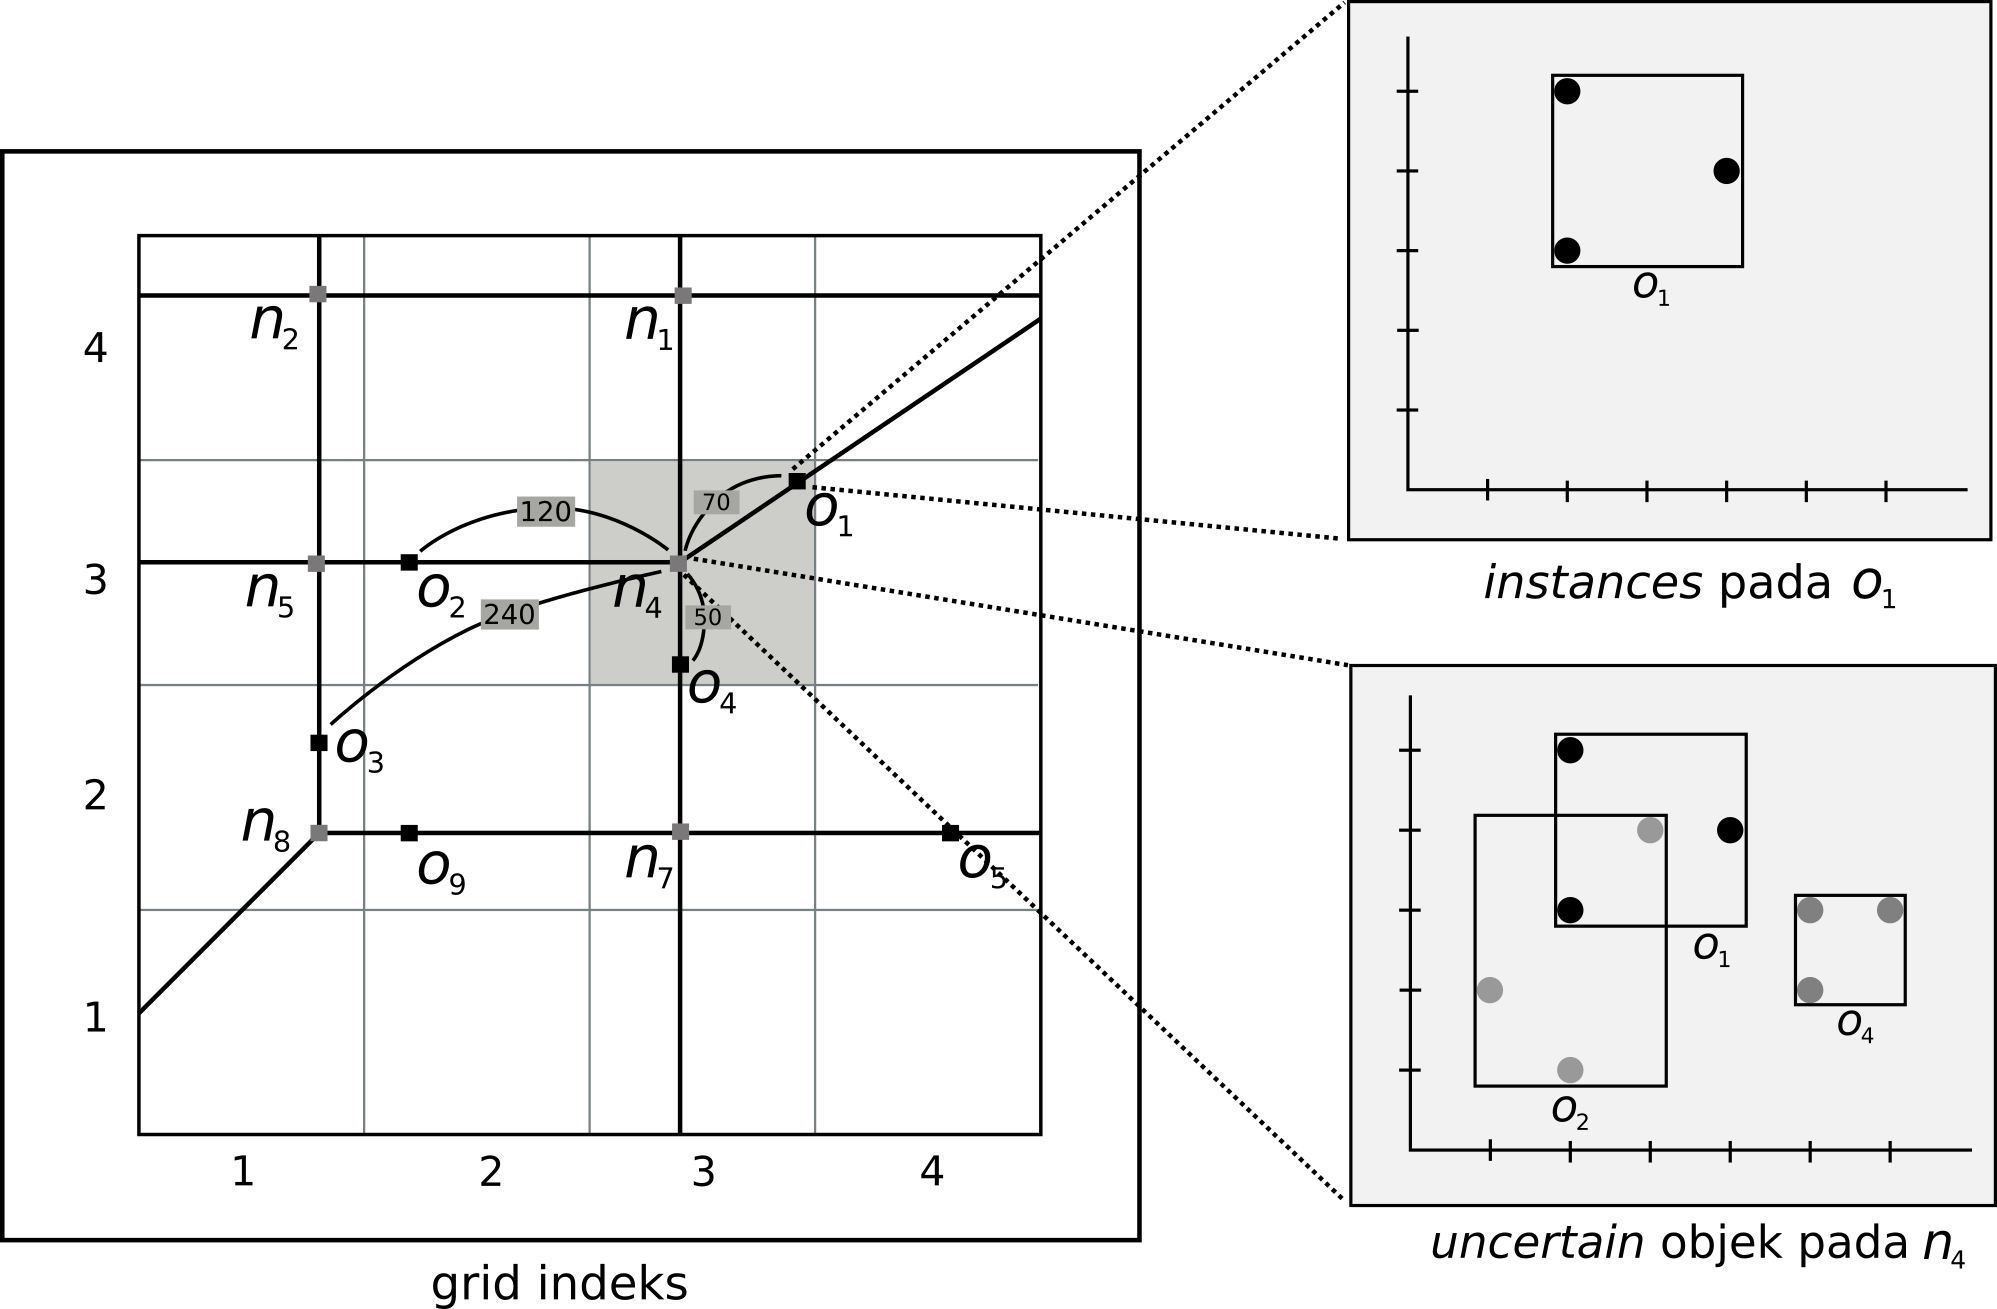
\includegraphics[width=9cm]{img/struktur-data.png}
	\caption{Struktur data grid indeks}
	\label{fig:grid}
\end{figure}

Perhatikan struktur tabel \textit{node} pada Tabel \ref{tab:node}. Setiap \textit{node} yang terdapat pada grid menyimpan koordinat $ x $, koordinat $ y $, struktur R-Tree \textit{SW-Tree}. Struktur R-Tree digunakan untuk menyimpan dan mengolah objek-objek \textit{uncertain data} secara efisien. \textit{SW-Tree} hanya menampung objek-objek yang berjarak kurang dari sama dengan $ d_\varepsilon $. Jarak yang dimaksud adalah total panjang \textit{edge}/jalan dari \textit{node} menuju objek. Pada dasarnya, \textit{SW-Tree} adalah struktur data R-Tree yang dimodifikasi agar dapat memproses \textit{uncertain data} dalam bentuk SW(\textit{sliding-window}). Terakhir, objek yang disimpan pada setiap \textit{node} tersebut diberi informasi tambahan (\textit{metadata}) agar algoritme tidak melakukan proses yang sama berulang-ulang.

\begin{table}[htbp]
	\caption{Node}
	\begin{center}
		\begin{tabular}{| p{2cm} | p{5cm} |}
			\hline
			\textbf{Atribut} & \textbf{Deskripsi} \\ \hline
			$ id $ & ID \textit{node} \\ \hline
			$ x $ & Koordinat X \\ \hline
			$ y $ & Koordinat Y \\ \hline
			\textit{SW-Tree} & Struktur RTree untuk menyimpan dan mengolah \textit{uncertain data} \\ \hline
			$ M $ & Tabel \textit{metadata} dari objek-objek yang disimpan \\ \hline
		\end{tabular}
		\label{tab:node}
	\end{center}
\end{table}

Perhatikan tabel \textit{edge} pada Tabel \ref{tab:edge}. Tabel \textit{edge} menyimpan $ n_i $ sebagai ID dari salah satu node, $ n_j $ sebagai ID dari \textit{node} lainnya, $ len $ sebagai panjang \textit{edge} tersebut, dan \textit{objects}. Atribut \textit{objects} pada \textit{edge} adalah semua objek yang berada pada \textit{edge} tersebut.

\begin{table}[htbp]
	\caption{Metadata}
	\begin{center}
		\begin{tabular}{| p{2cm} | p{5cm} |}
			\hline
			\textbf{Atribut} & \textbf{Deskripsi} \\ \hline
			$ id $ & ID dari objek \\ \hline
			$ d $ & Jarak objek dari \textit{node n} \\ \hline
			$ skyProb $ & Probabilitas objek menjadi bagian dari $ SP $ \\ \hline
			$ isImpossible $ & Tanda jika objek tidak dapat menjadi bagian dari $ SP $ \\ \hline
		\end{tabular}
		\label{tab:metadata}
	\end{center}
\end{table}

Tabel \ref{tab:metadata} menyimpan data yang melekat pada objek ketika objek sudah masuk pada  \textit{edge} $ e $. Tabel tersebut menyimpan jarak \textit{d}, yaitu jarak antara \textit{node} dengan objek. Dengan adanya \textit{d}, algoritme yang diusulkan tidak menggunakan komputasi \textit{shortest-path}. \textit{skyProb} menyimpan probabilitas objek menjadi bagian dari \textit{SP} dan \textit{skyProb} bernilai $ 0 \le skyProb \le 1 $. Terakhir, \textit{isImpossible} adalah \textit{flag} yang menjadi tanda apabila objek tidak lagi dapat menjadi bagian dari \textit{SP}.

\begin{table}[htbp]
	\caption{Edge}
	\begin{center}
		\begin{tabular}{| p{2cm} | p{5cm} |}
			\hline
			\textbf{Atribut} & \textbf{Deskripsi} \\ \hline
			$ id $ & ID \textit{edge} \\ \hline
			$ n_i $ & ID \textit{node} salah satu ujung \\ \hline
			$ n_j $ & ID \textit{node} ujung yang lain \\ \hline
			$ len $ & Panjang \textit{edge} \\ \hline
			$ objects $ & Kandidat \textit{skyline point}, yaitu semua objek yang berada pada \textit{edge} tersebut \\
			\hline
		\end{tabular}
		\label{tab:edge}
	\end{center}
\end{table}


\subsection{Metode Pemrosesan $ CSd_\varepsilon-SQ $}
Artikel ini mengusulkan metode \textit{Continuous Streaming distance-based Skyline Query} ($ CSd_\varepsilon-SQ $). Pencarian titik \textit{skyline} pada jaringan jalan raya menggunakan algoritme $ Cd_\varepsilon-SQ $\cite{continuousdbased}. Untuk mencari \textit{skyline point}, $ SP $ dari suatu titik \textit{query}, komputasi dilakukan untuk mencari semua objek yang memiliki jarak kurang dari sama dengan $ d_\varepsilon $ dari titik \textit{query} tersebut. Dari objek-objek tersebut, metode ini mencari objek-objek yang tidak didominasi oleh objek lain, objek-objek tersebut dinamai \textit{GSP}(\textit{Global Skyline Points}).


\begin{figure}[H]
	\begin{algorithm}[H]
		\label{algo:gsp}
		\caption{DetermineGSP}
		\begin{algorithmic}[1]
			\State \textbf{Input: }grid index \textit{G}, a distance $ d_\varepsilon $, uncertain data object $ X $, action(insertion/deletion)
			\State \textbf{Output: }an updated grid index \textit{G}
			\State create empty queue $ Q $
			\State create temporary graph $ Gr $
			\State access edge $ e $ enclosing $ X $ and enqueue $ n_i  $ and $ n_j $
			\State enqueue $ n_i $ and $ n_j $ with each distance
			\While{$ Q $ is not empty}
			\State sort Q by distance from $ X $
			\State dequeue $ Q $ as $ n $
			\If{$d_{n, X} \le d_\varepsilon $}
			\State insert grid enclosing $ n $ to $ Gr $
			\If{action is insertion}
			call $ Insertion() $
			\Else
			$ $ call $ Deletion() $
			\EndIf
			\ForAll{node $ m $ as neighbor of $ n $}
			\If{$ m $ has not visited}
			\State enqueue $ m $ with it's distance
			\State mark $ m $ as visited
			\EndIf
			\EndFor
			\EndIf
			\EndWhile
			\ForAll{edge $ e $ which has updated $ n_s $ or $ n_e $ in $ Gr $}
			\State find GSP as $ gsp $
			\State call \textit{ComputeTurningPoint($ gsp $)}
			\EndFor
		\end{algorithmic}
	\end{algorithm}
	\caption{Algoritme \textit{DetermineGSP}}
\end{figure}

Untuk menentukan \textit{GSP} pada \textit{uncertain data streaming}, algoritme yang digunakan adalah metode EPSU\cite{effectiveprob}. Metode ini menggunakan struktur data grid indeks agar algoritme hanya memproses data yang dibutuhkan saja. Agar pemrosesan \textit{uncertain data} dapat dilakukan secara efisien, penelitian ini menggunakan struktur data R-Tree dan disimpan pada setiap \textit{node}.

\begin{figure}[H]
	\centering
	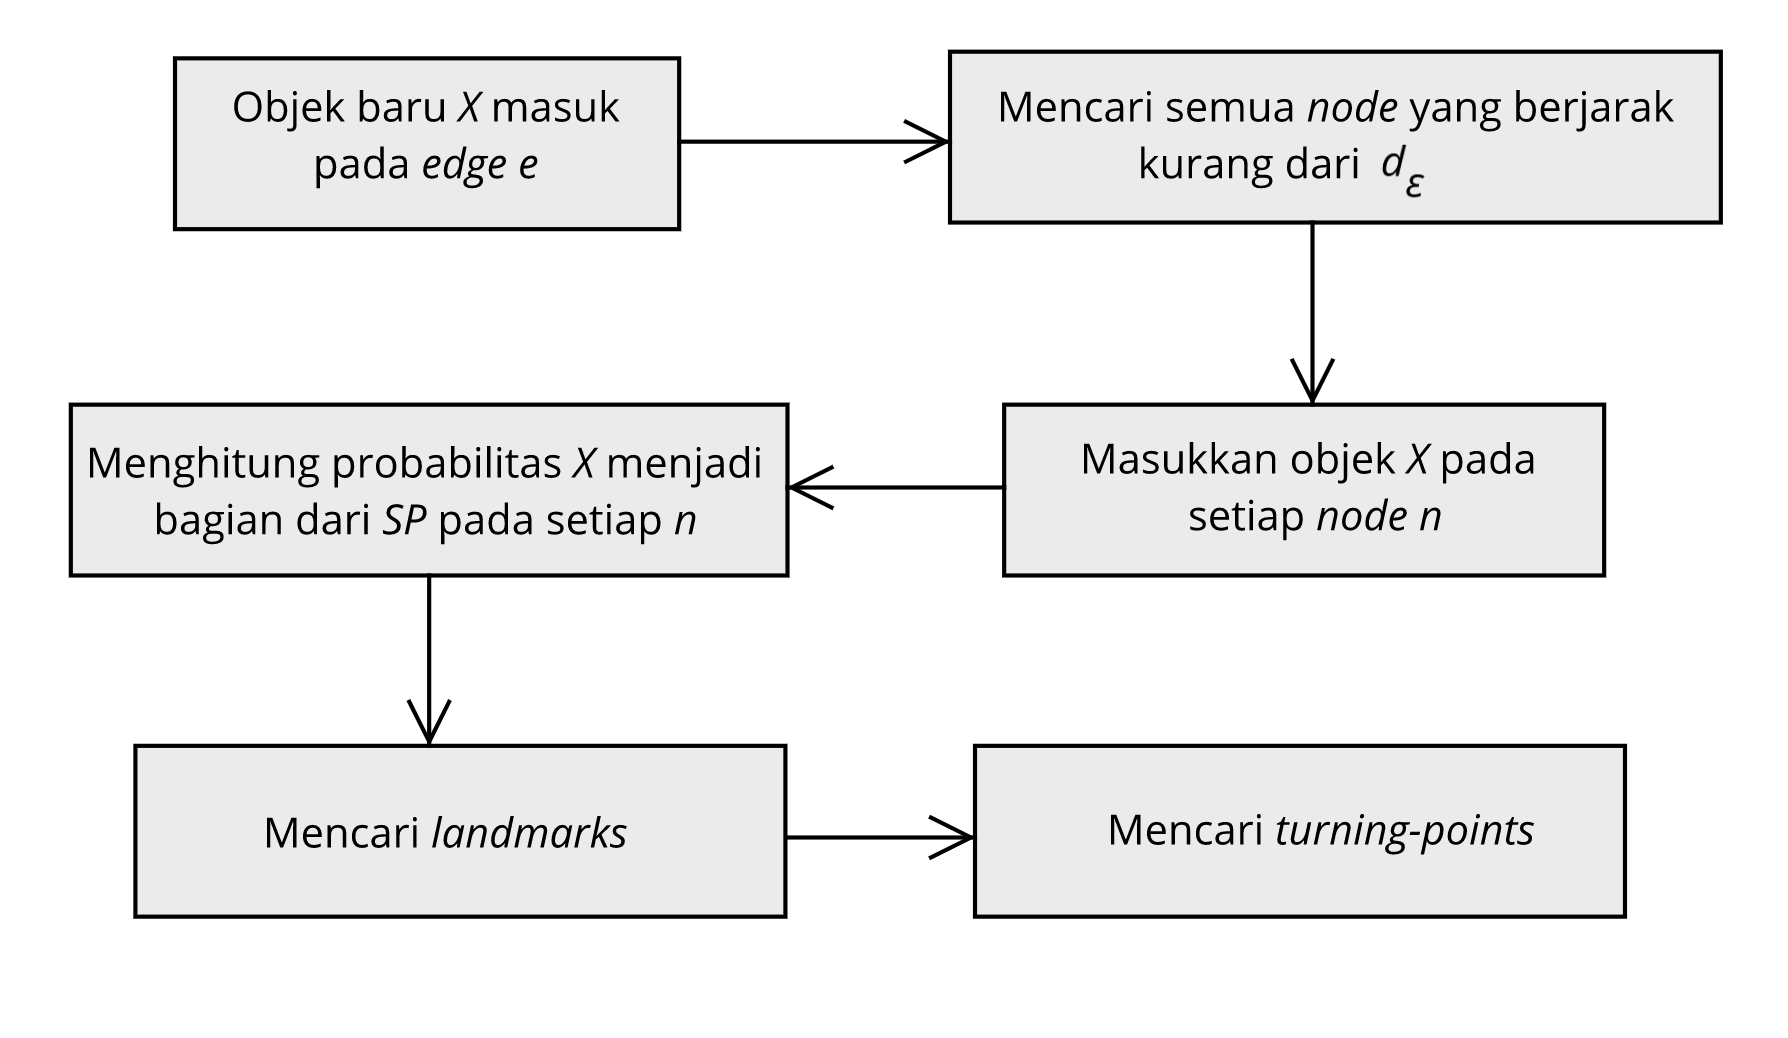
\includegraphics[width=8cm]{img/alur.png}
	\caption{Alur pemrosesan}
	\label{fig:alur}
\end{figure}

Perhatikan Gambar \ref{fig:alur} dan Gambar \ref{fig:alur1-2}, saat objek $ X $ yang masuk dari \textit{stream} pada suatu \textit{edge} yang terdapat pada struktur Grid, algoritme BFS mencari semua \textit{node} yang berjarak kurang dari $ d_\varepsilon $ dari objek $ X $, $ d_{X, n} \le d_\varepsilon $.

\begin{figure}[H]
	\centering
	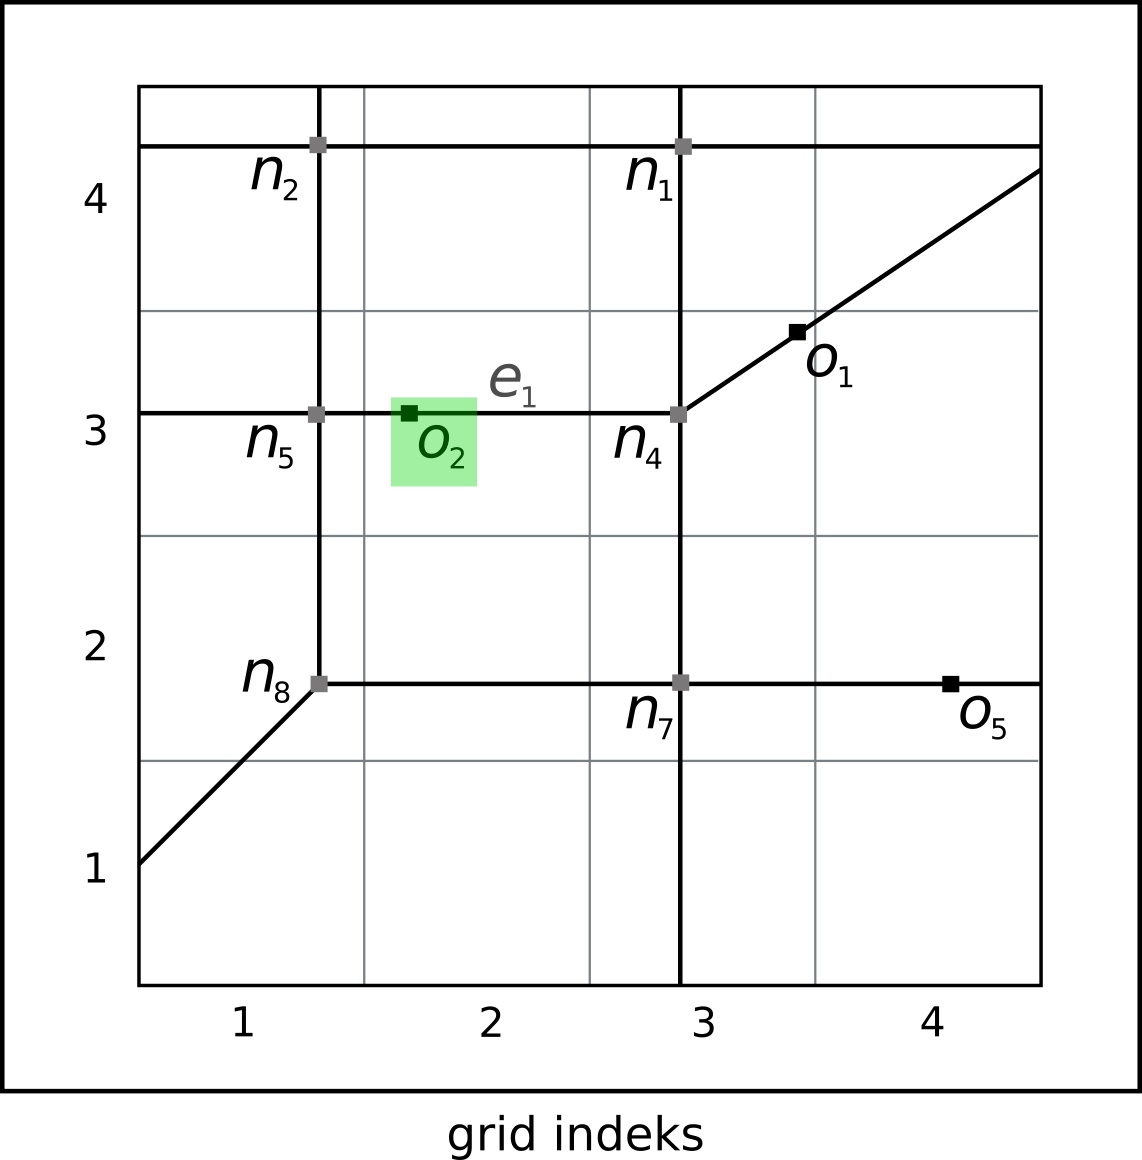
\includegraphics[width=5cm]{img/alur/alur1.png}
	\caption{Objek masuk pada grid indeks}
	\label{fig:alur1-2}
\end{figure}

Kemudian objek $ X $ dimasukkan pada struktur data R-Tree yang terdapat pada masing-masing \textit{node} menggunakan algoritme \textit{Insertion}. Setiap objek $ X $ bertahan pada Grid hanya dalam interval waktu yang sama \textit{t}. Jika objek $ X $ sudah kadaluarsa, objek dikeluarkan dari \textit{node} dengan algoritme \textit{Deletion}.

	
	\begin{figure}[H]
		\begin{algorithm}[H]
			\label{algo:insertion}
			\caption{\textit{Insertion}}
			\begin{algorithmic}[1]
				\State \textbf{Input: } uncertain data object $ X $, threshold $ p $
				\For{each object Q overlapped with \textit{PDR(X)}}
				\If{\textit{MBR(Q) is within \textit{DDR(X)}}}
				\State mark \textit{Q} as impossible object
				\Else
				\If{$ \sum_{\textit{q in MBR(Q)$ \cap $DDR(X)}} Pr(q) > (1 - p)$}
				\State mark \textit{Q} as as impossible object
				\Else 
				\State update SkyPr(\textit{Q}) with \textit{X}
				\EndIf
				\EndIf
				\EndFor
				\State compute SkyPr(\textit{X}) with objects overlapped with \textit{PDD(X)}
				\State insert \textit{X} into \textit{SW-Tree}
			\end{algorithmic}
		\end{algorithm}
		\caption{Algoritme \textit{Insertion}}
	\end{figure}

	\begin{figure}[H]
		\begin{algorithm}[H]
			\label{algo:deletion}
			\caption{\textit{Deletion}}
			\begin{algorithmic}[1]
				\State \textbf{Input: }expired uncertain data $ U $, threshold $ p $
				\For{each object \textit{Q} overlapped with \textit{PDR(X) and not marked}}
				\State update SkyPr(\textit{Q}) with removal of \textit{X}
				\EndFor
				\State Remove X from \textit{SW-Tree}
			\end{algorithmic}
		\end{algorithm}
		\caption{Algoritme \textit{Deletion}}
	\end{figure}


Setelah objek masuk pada semua \textit{node} $ n $ $ d_{X, n} \le d_\varepsilon $, proses pencarian \textit{landmark} dilakukan sebagai dasar pencarian \textit{turning-point}. Masukan dari proses pencarian \textit{Landmark} yaitu \textit{GSP}. \textit{GSP} adalah objek-objek yang menjadi $ SP^\varepsilon $ yang terdapat pada $ n_s $ dan $ n_e $ dan objek-objek yang terdapat pada edge $ e $. Terakhir, penentuan \textit{turning-point} dilakukan pada setiap \textit{edge} yang berhubungan dengan $ n $. Hasil akhir dari proses ini adalah \textit{turning-point}.

\begin{figure}
	\centering
	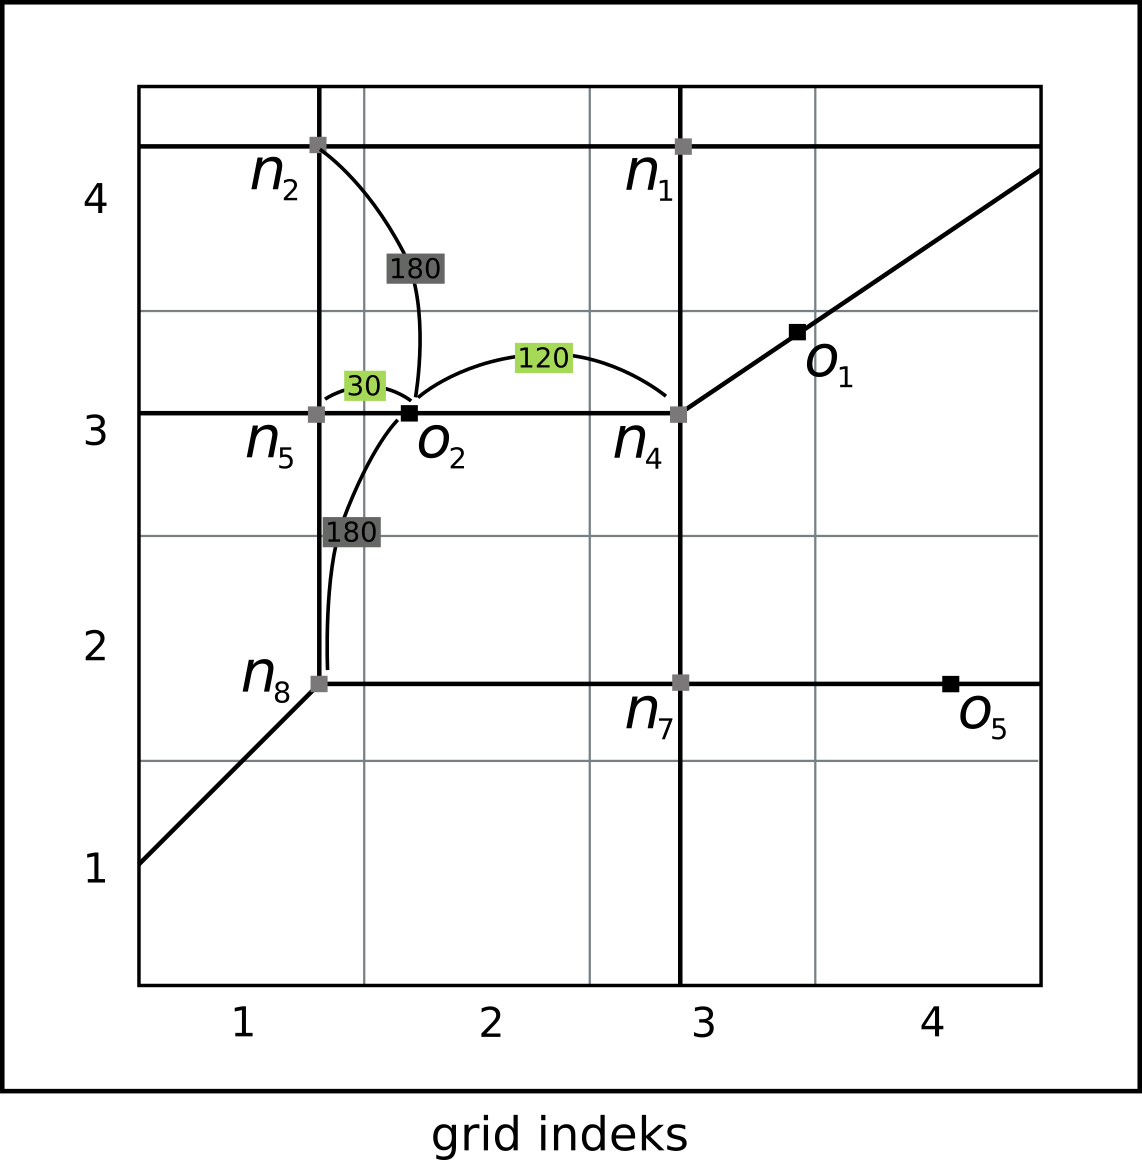
\includegraphics[width=5cm]{img/alur/alur3.png}
	\caption{Dengan $ d_\varepsilon $=150, $ o_2 $ hanya masuk pada \textit{node} $ n_4 $ dan $ n_5 $}
	\label{fig:alur3}
\end{figure}

\begin{figure}
	\centering
	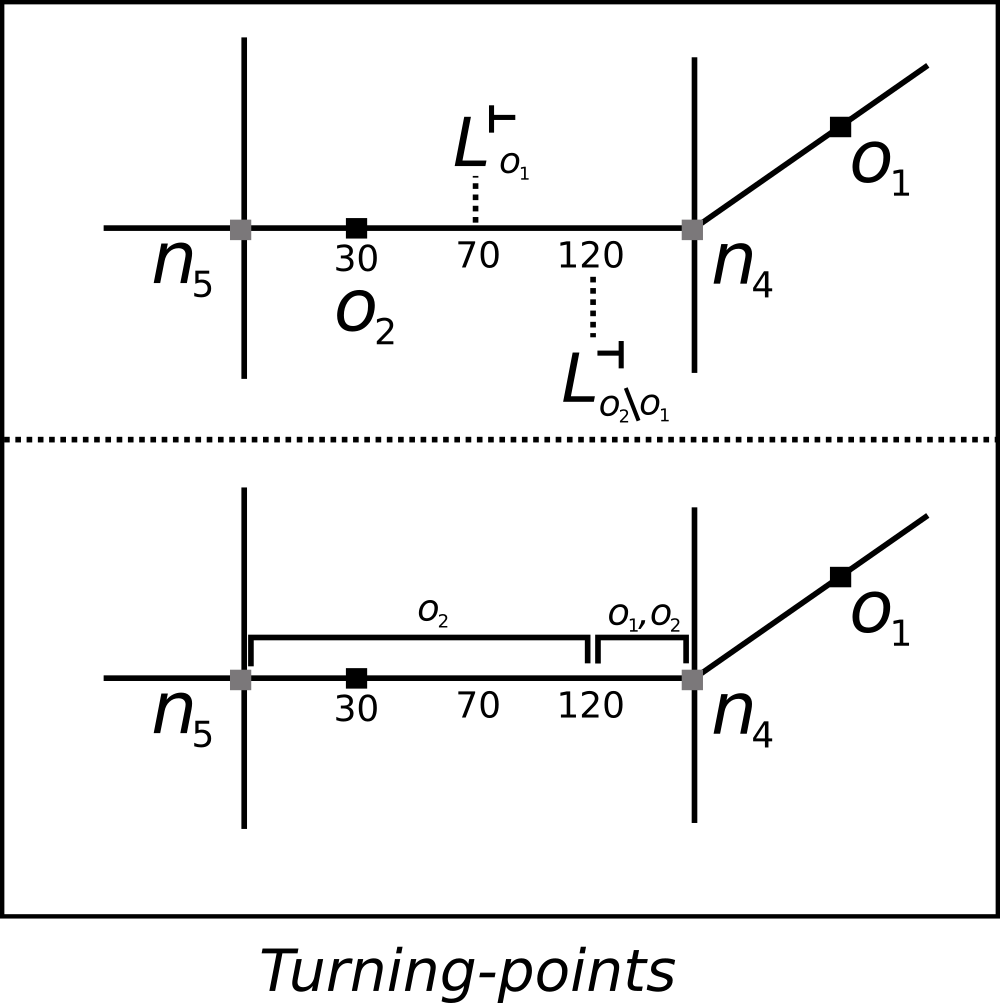
\includegraphics[width=5cm]{img/alur/alur6.png}
	\caption{Atas: \textit{landmark} yang didapat dari \textit{edge}. Bawah: \textit{turning-point} didapat dari \textit{landmark}}.
	\label{fig:alur4-5}
\end{figure}

Suatu edge $ e $ pada jaringan jalan raya memiliki dua ujung \textit{node}, yaitu \textit{node} ujung awal $ n_s $ dan \textit{node} ujung akhir $ n_e $. Setiap \textit{node} memiliki objek dan terhubung dengan \textit{edge}. Dari proses  \textit{Skyline} \textit{edge} \textit{e} direpresentasikan dalam bentuk interval beserta \textit{SP} yang terdapat pada masing-masing interval. Antara interval satu dengan interval lain terdapat pergantian objek yang menjadi \textit{SP}. Titik pergantian \textit{SP} ini diistilahkan dengan \textit{turning-point}.

\begin{figure}
	\begin{algorithm}[H]
		\label{compute_turning_point}
		\caption{ComputeTurningPoint}
		\begin{algorithmic}[1]
			\State \textbf{Input: }threshold $ p $, a distance $ d_\varepsilon $, a set \textit{GSP}, an edge \textit{e} connecting two nodes $ n_s $ and $ n_e $
			\State \textbf{Output:} A set of tuples in form of $ < [n_i, n_j], SP^\varepsilon >$ where $ SP^\varepsilon $ is the $ d_\varepsilon-SP $ set between $ [n_i, n_j] $
			\State create an empty queue Q
			\For{object \textit{o} $ \in $ \textit{GSP}}
			\State determine \textit{o}'s landmarks $ L_o^\vdash $ and $ L_o^\dashv $
			\If{$ L_o^\vdash $ is on \textit{e}}
			insert $ L_o^\vdash $ into \textit{Q}
			\EndIf
			\If{$ L_o^\dashv $ is on \textit{e}}
			insert $ L_o^\dashv $ into \textit{Q}
			\EndIf
			\For{object \textit{o'} $ \in (GSP-\{o\}) \cap \sum_{\textit{q in MBR(o')$ \cap $DDR(o)}} Pr(q) > (1 - p) $}
			\State determine \textit{o}'s landmarks $ L_o^\vdash $ or $ L_o^\dashv $
			\If{ $ L_{o \setminus o'}^\vdash $ is on $ e $ and $ L_o^\vdash $ is closer to $ n_s $ than $ L_{o \setminus o'}^\vdash $}
			\State insert $ L_{o \setminus o'}^\vdash $ into \textit{Q}
			\EndIf
			\If{ $ L_{o \setminus o'}^\dashv $ is on $ e $ and $ L_{o \setminus o'}^\dashv $ is closer to $ n_s $ than $ L_{o}^\dashv $}
			\State insert $ L_{o \setminus o'}^\dashv $ into \textit{Q}
			\EndIf
			\EndFor
			\EndFor
			\State sort landmarks in Q in ascending order of their distances to $ n_s $
			
			\State /* determining the result turning points */
			\While{\textit{Q} is not empty}
			\State dequeue $ o.L $
			\Switch{$ o.L $}
			\Case{$ L_o^\vdash $}
			\If{there is no $ L_{o' \setminus o}^\dashv $}
			\State return $ < [n_i, L_o^\vdash], SP^\varepsilon >, n_i =  L_o^\vdash $,
			\State and add \textit{o} into $ SP^\varepsilon $
			\EndIf
			\EndCase
			\Case{$ L_o^\dashv $}
			\If{$ o \in SP^\varepsilon $}
			\State return $ < [n_i, L_o^\dashv], SP^\varepsilon >, n_i =  L_o^\dashv $,
			\State and remove \textit{o} from $ SP^\varepsilon $
			\EndIf
			\EndCase
			\Case{$ L_{o \setminus o'}^\vdash $}
			\If{$ o \in SP^\varepsilon $ and $ o' \in SP^\varepsilon $}
			\State return $ < [n_i, L_{o \setminus o'}^\vdash], SP^\varepsilon >, n_i = L_{o \setminus o'}^\vdash $,
			\State and remove \textit{o'} from $ SP^\varepsilon $
			\EndIf
			\EndCase
			\Otherwise{}
			\If{$ o \in SP^\varepsilon $ and there is no $ L_{o'' \setminus o'}^\dashv \in Q $ }
			\State return $ < [n_i, L_{o \setminus o'}^\dashv], SP^\varepsilon >, $
			\State $ n_i = L_{o \setminus o'}^\dashv, $ and add \textit{o'} into $ SP^\varepsilon $
			\EndIf
			\EndOtherwise
			\EndSwitch
			\EndWhile
		\end{algorithmic}
	\end{algorithm}
	\caption{Algoritme \textit{Compute Turning Point}}
\end{figure}

Algoritma pada Gambar 11 mengilustrasikan penentuan \textit{landmark} pada \textit{edge} $ e $ yang memiliki \textit{node} awal $ n_s $ dan \textit{node} lainnya $ n_e $. Queue $ Q $ dibuat untuk menampung \textit{landmark}. Penentuan landmark ini berdasarkan pada objek-objek yang menjadi anggota dari \textit{GSP}. Setelah mendapatkan semua landmark, \textit{queue} $ Q $ diurutkan berdasarkan jarak terdekat dari \textit{node} $ n_s $.

Setelah semua \textit{landmark} didapatkan, pencarian \textit{turning-point} dilakukan. \textit{Turning-point} ini adalah hasil dari algoritma. \textit{Turning-point} berupa sekumpulan \textit{tuple} yang merepresentasikan interval awal $ n_i $, interval akhir $ n_e $, dan objek-objek yang menjadi $ SP $ pada interval tersebut $ SP^\varepsilon $.

\section{Uji Coba}
Uji coba dilakukan pada jaringan jalan raya California\cite{ontrip} dengan \textit{node} sebanyak 8716 dan \textit{edge} sebanyak 9077. Algoritma diimplementasikan menggunakan bahasa Scala dengan \textit{memory heap} sejumlah 4 GB. Pengujian dilakukan pada komputer dengan \textit{Processor} Intel(R) Core(TM) i3-5010U CPU @ 2.10GHz x 4 dan RAM 6 GB. Pengujian dilakukan untuk mengetahui performa dengan menggunakan waktu komputasi dan untuk mengetahui penggunaan memori pada setiap eksekusi. Uji coba juga dilakukan pada tiga jenis data, yaitu data \textit{independent}, \textit{correlated}, dan \textit{anticorrelated}.

\begin{table}[htbp]
	\caption{Variasi pengujian}
	\begin{center}
		\begin{tabular}{| l | l | l |}
			\hline
			\textbf{Parameter} & \textbf{\textit{Default}} & \textbf {Rentang} \\ \hline
			Jumlah sel grid & $ 256^2 $ & $ 32^2 $, $ 64^2 $, $ 128^2 $, $ 256^2 $, $ 512^2 $ \\ \hline
			Jumlah objek (K) & 5 & 0.1, 1, 5, 10, 20 \\ \hline
			Jumlah \textit{instance} tiap objek & 50 & 10, 50, 100, 200, 400 \\ \hline
			$ d_\varepsilon $ (\%) & 1 & 0.1, 0.5, 1, 2, 3 \\ \hline
			Dimensi data & 2 & 2, 3, 4, 5, 6 \\ \hline
		\end{tabular}
		\label{tab:uji}
	\end{center}
\end{table}

\begin{figure}
	\centering
	\begin{tikzpicture}
	\begin{axis}[
	height=6cm,
	xlabel={Jumlah sel grid},
	ylabel={waktu komputasi (detik/operasi)},
	ymin=0, ymax=1,
	xmin=0, xmax=10,
	xtick={1, 3, 5, 7, 9},
	xticklabels={$ 32^2 $, $ 64^2 $, $ 128^2 $, $ 256^2 $, $ 512^2 $},
	legend pos=north east,
	ymajorgrids=true,
	grid style=dashed,
	]
	
	\addplot[
	color=blue,
	mark=square,
	]
	coordinates {
		(1, 0.198035104400913)(3, 0.19713375528914)(5, 0.214094556217187)(7, 0.177597533827906)(9, 0.213052689078089)
	};
	\addlegendentry{$ CSd_\varepsilon $}
	
	\end{axis}
	\end{tikzpicture}
	\caption{Pengaruh jumlah sel terhadap waktu komputasi tiap operasi dalam satuan detik}\label{fig:uji-g}
\end{figure}

\begin{figure}
	\centering
	\begin{tikzpicture}
	\begin{axis}[
	height=6cm,
	xlabel={Jumlah sel grid},
	ymin=0, ymax=500,
	ylabel={penggunaan memori (MB)},
	xmin=0, xmax=10,
	xtick={1, 3, 5, 7, 9},
	xticklabels={$ 32^2 $, $ 64^2 $, $ 128^2 $, $ 256^2 $, $ 512^2 $},
	legend pos=south east,
	ymajorgrids=true,
	grid style=dashed,
	]
	
	\addplot[
	color=blue,
	mark=square,
	]
	coordinates {
		(1, 205)(3, 245)(5, 222)(7, 209)(9, 214)
	};
	\addlegendentry{$ CSd_\varepsilon $}
	
	\end{axis}
	\end{tikzpicture}
	\caption{Pengaruh jumlah sel grid terhadap penggunaan memori dalam satuan megabita}\label{fig:uji-g-mem}
\end{figure}

Jumlah sel tidak banyak mempengaruhi penggunaan memori dan waktu komputasi. Hal ini dikarenakan adanya \textit{trade-off} antara proses memuat data dengan komputasi. Grid indeks yang memiliki sel sedikit menjadikan data yang dimuat lebih banyak sehingga menjadikan data yang diproses labih banyak. Tetapi di sisi lain, sistem tidak banyak mencari data secara berulang-ulang karena setiap sel sudah mengaver area yang besar. Sedangkan grid indeks yang memiliki sel yang banyak menjadikan proses komputasi lebih efisien karena melibatkan data yang lebih sedikit. Tetapi di sisi lain, sistem harus melakukan pencarian data berulang-ulang karena sedikitnya data yang didapat pada setiap sel.

\begin{figure}
	\centering
	\begin{tikzpicture}
	\begin{axis}[
	width=6cm,
	xlabel={Jumlah objek (k)},
	ymode=log,
	ylabel={waktu komputasi (detik/operasi)},
	xmin=0, xmax=10,
	xtick={1, 3, 5, 7, 9},
	xticklabels={0.1, 1, 5, 10, 20},
	legend pos=south east,
	ymajorgrids=true,
	grid style=dashed,
	]
	
	\addplot[
	color=blue,
	mark=square,
	]
	coordinates {
		(1,0.027)(3, 0.054)(5, 0.24)(7, 0.527)(9, 1.062)
	};
	\addlegendentry{$ CSd_\varepsilon $}
	
	\addplot[
	color=red,
	mark=x,
	]
	coordinates {
		(1,63)(3, 64)(5, 68)(7, 90)(9, 167)
	};
	\addlegendentry{\textit{Naive}}
	
	\end{axis}
	\end{tikzpicture}
	\caption{Pengaruh jumlah objek terhadap waktu komputasi tiap operasi dalam satuan detik}\label{fig:uji-n}
\end{figure}

Ketika jumlah objek bertambah, waktu pemrosesan juga bertambah, hal ini dikarenakan bertambahnya objek yang terdapat pada \textit{node}. Dengan bertambahnya objek pada \textit{node}, algoritme perlu membandingkan dengan objek yang lebih banyak untuk mencari probabilitas masing-masing objek menjadi \textit{SP}.

\begin{figure}
	\centering
	\begin{tikzpicture}
	\begin{axis}[
	width=6cm,
	xlabel={Jumlah objek (k)},
	ymode=log,
	ylabel={penggunaan memori (MB)},
	xmin=0, xmax=10,
	xtick={1, 3, 5, 7, 9},
	xticklabels={0.1, 1, 5, 10, 20},
	legend pos=south east,
	ymajorgrids=true,
	grid style=dashed,
	]
	
	\addplot[
	color=blue,
	mark=square,
	]
	coordinates {
		(1, 16)(3, 41)(5, 328)(7, 367)(9, 375)
	};
	\addlegendentry{$ CSd_\varepsilon $}
	
	\addplot[
	color=red,
	mark=x,
	]
	coordinates {
		(1, 77062)(3, 79292)(5, 78801)(7, 73392)(9, 67442)
	};
	\addlegendentry{\textit{Naive}}
	
	\end{axis}
	\end{tikzpicture}
	\caption{Pengaruh jumlah objek terhadap penggunaan memori dalam satuan megabita}\label{fig:uji-n-mem}
\end{figure}

Terkait penggunaan memori, metode \textit{naive} membutuhkan memori yang sangat banyak karena banyaknya \textit{node} yang perlu diproses menggunakan algoritme \textit{shortest-path}. Sedangkan metode $ CSd_\varepsilon-SQ$ membutuhkan memori yang tidak banyak karena hanya menggunakan data \textit{node} yang diperlukan saja dengan struktur grid.

Jumlah \textit{instance} pada objek mempengaruhi waktu komputasi dan penggunaan memori. Hal ini dikarenakan proses penghitungan probabilitas melibatkan \textit{instances} di objek. Dari sisi memori, banyaknya \textit{instance} membuat sistem harus mengalokasikan memori lebih untuk proses penyimpanan dan komputasi.

\begin{figure}
	\centering
	\begin{tikzpicture}
	\begin{axis}[
	width=6cm,
	xlabel={\textit{instances}},
	ymode=log,
	ylabel={waktu komputasi (detik/operasi)},
	xmin=0, xmax=10,
	xtick={1, 3, 5, 7, 9},
	xticklabels={10, 50, 100, 150, 200},
	legend pos=south east,
	ymajorgrids=true,
	grid style=dashed,
	]
	
	\addplot[
	color=blue,
	mark=square,
	]
	coordinates {
		(1, 0.033)(3, 0.229)(5, 0.979)(7, 3)(9, 5.736)
	};
	\addlegendentry{$ CSd_\varepsilon $}
	
	\addplot[
	color=red,
	mark=x,
	]
	coordinates {
		(1, 67)(3, 70)(5, 74)(7, 133)(9, 132)
	};
	\addlegendentry{\textit{Naive}}
	
	\end{axis}
	\end{tikzpicture}
	\caption{Pengaruh jumlah \textit{instance} terhadap waktu komputasi tiap operasi dalam satuan detik}\label{fig:uji-np}
\end{figure}

Pada metode \textit{naive}, objek perubahan waktu komputasi terlihat ketika jumlah \textit{instance} diatas 100. Hal ini dikarenakan waktu komputasi lebih banyak digunakan untuk penghitungan jarak terpendek dari setiap \textit{node} ke objek, sehingga jumlah \textit{instance} yang sedikit tidak berpengaruh banyak terhadap waktu komputasi.

\begin{figure}
	\centering
	\begin{tikzpicture}
	\begin{axis}[
	width=6cm,
	xlabel={\textit{instances}},
	ymode=log,
	ylabel={penggunaan memori (MB)},
	xmin=0, xmax=10,
	xtick={1, 3, 5, 7, 9},
	xticklabels={10, 50, 100, 150, 200},
	legend pos=south east,
	ymajorgrids=true,
	grid style=dashed,
	]
	
	\addplot[
	color=blue,
	mark=square,
	]
	coordinates {
		(1, 41)(3, 139)(5, 4874)(7, 11213)(9, 32760)
	};
	\addlegendentry{$ CSd_\varepsilon $}
	
	\addplot[
	color=red,
	mark=x,
	]
	coordinates {
		(1, 73772)(3, 81068)(5, 79448)(7, 71448)(9, 58597)
	};
	\addlegendentry{\textit{Naive}}
	
	\end{axis}
	\end{tikzpicture}
	\caption{Pengaruh jumlah \textit{instance} terhadap penggunaan memori dalam satuan megabita}\label{fig:uji-np-mem}
\end{figure}

Jarak $ d_\varepsilon $ sangat mempengaruhi \textit{performance} karena $ d_\varepsilon $ menentukan jarak terjauh \textit{node} yang dapat menyimpan objek baru. Dengan bertambahnya nilai $ d_\varepsilon $, objek dapat menjangkau lebih banyak \textit{node}. Dengan demikian, objek yang ditampung pada \textit{node} menjadi semakin banyak. Dengan semakin banyaknya objek, proses penghiungan probabilitas \textit{skyline} menjadi semakin lama karena harus menghitung banyak objek. Pada $ CSd_\varepsilon-SQ$, semakin besar nilai $ d_\varepsilon $, semakin banyak grid yang diakses sehingga membutuhkan waktu yang lebih banyak. Pada metode \textit{naive}, terdapat perubahan waktu komputasi yang signifikan ketika nilai $ d_\varepsilon $ diatas 1.

\begin{figure}[H]
	\centering
	\begin{tikzpicture}
	\begin{axis}[
	width=6cm,
	xlabel={$ d_\varepsilon $},
	ymode=log,
	ylabel={waktu komputasi (detik/operasi)},
	xmin=0, xmax=10,
	xtick={1, 3, 5, 7, 9},
	xticklabels={0.1, 0.5, 1, 2, 3},
	legend pos=south east,
	ymajorgrids=true,
	grid style=dashed,
	]
	
	\addplot[
	color=blue,
	mark=square,
	]
	coordinates {
		(1, 0.009)(3, 0.052)(5, 0.24)(7, 1.592)(9, 9.667)
	};
	\addlegendentry{$ CSd_\varepsilon $}
	
	\addplot[
	color=red,
	mark=x,
	]
	coordinates {
		(1, 64)(3, 67)(5, 68)(7, 216)(9, 490)
	};
	\addlegendentry{\textit{Naive}}
	
	\end{axis}
	\end{tikzpicture}
	\caption{Pengaruh $ d_\varepsilon $ terhadap waktu komputasi tiap operasi dalam satuan detik}\label{fig:uji-d}
\end{figure}

Penggunaan memori sangat tergantung dari jumlah objek yang diproses. Nilai $ d_\varepsilon $ yang besar menjadikan objek yang diproses semakin banyak karena setiap \textit{node} memiliki jangkauan yang lebih jauh. Banyaknya objek yang diproses menjadikan penggunaan memori semakin besar.

\begin{figure}[H]
	\centering
	\begin{tikzpicture}
	\begin{axis}[
	width=6cm,
	xlabel={$ d_\varepsilon $},
	ymode=log,
	ylabel={penggunaan memori (MB)},
	xmin=0, xmax=10,
	xtick={1, 3, 5, 7, 9},
	xticklabels={0.1, 0.5, 1, 2, 3},
	legend pos=south east,
	ymajorgrids=true,
	grid style=dashed,
	]
	
	\addplot[
	color=blue,
	mark=square,
	]
	coordinates {
		(1, 12)(3, 122.7)(5, 328)(7, 5932)(9, 37507)
	};
	\addlegendentry{$ CSd_\varepsilon $}
	
	\addplot[
	color=red,
	mark=x,
	]
	coordinates {
		(1, 74387)(3, 72904)(5, 78801)(7, 126323)(9, 230699)
	};
	\addlegendentry{\textit{Naive}}
	
	\end{axis}
	\end{tikzpicture}
	\caption{Pengaruh $ d_\varepsilon $ terhadap penggunaan memori dalam satuan megabita}\label{fig:uji-d-mem}
\end{figure}

\section{Kesimpulan}
Pada bab ini dijelaskan mengenai kesimpulan dan saran dari hasil uji coba yang telah dilakukan.

Dari proses desain hingga uji coba, dapat diambil beberapa hasil sebagai berikut:

\begin{enumerate}
	\item Artikel ini mengusulkan struktur data grid indeks dan metode $ CSd_\varepsilon $ untuk pengolahan \textit{skyline query} pada \textit{uncertain data streaming} oleh titik bergerak dan objek tidak bergerak. Struktur data grid indeks memecah struktur data graf tradisional menjadi sel-sel yang berisi \textit{node}, \textit{edge}, dan objek. Penyimpanan objek dalam bentuk \textit{SW-Tree} pada setiap \textit{node} membuat proses komputasi lebih cepat.
	
	\item Biaya komputasi pada metode $ CSd_\varepsilon $ jauh lebih baik dibandingkan metode \textit{naive} dari sisi waktu komputasi dan penggunaan memori. Komputasi metode $ CSd_\varepsilon $ lebih cepat 600 kali dibandingkan metode \textit{naive}. Dari sisi penggunaan memori, metode $ CSd_\varepsilon $ lebih hemat 1500 kali dibandingkan metode \textit{naive}.
\end{enumerate}

Berikut beberapa saran terkait pengembangan struktur data dan algoritma lebih lanjut:

\begin{enumerate}
	\item Pendefinisian jarak $ d_\varepsilon $ dapat dilakukan secara dinamis. Apabila pencarian objek dengan jarak $ d_\varepsilon $ tidak menemukan hasil yang diminta, jarak $ d_\varepsilon $ dapat diperbesar secara dinamis hingga mendapatkan hasil yang sesuai.
	\item Pengembangan algoitma untuk memproses objek \textit{uncertain} yang dapat bergerak secara dinamis.
	\item Pada algoritme ini proses pembaruan \textit{instance} dari \textit{uncertain} objek dilakukan dengan menghapus dan menambahkan objek baru. Hal ini tentunya tidak efisien. Diperlukan algoritme pembaruan objek agar lebih efisien dalam hal waktu komputasi dan penggunaan memori.
\end{enumerate}

\begin{thebibliography}{00}

\bibitem{kmpp}
M. S. Islam and C. Liu, "Know Your Customer: Computing K-Most Promising Products," \textit{The VLDB Journal}, pp. 545–570, 2016.

\bibitem{dynamic-skyline}
D. Papadias, Y. Tao, G. Fu and B. Seeger, "Progressive Skyline Computation in Database Systems," \textit{ACM Transactions on Database Systems}, Vol. 30, No. 1, pp. 41–82, 2005.

\bibitem{reverse-skyline}
E. Dellis and B. Seeger, "Efficient Computation of Reverse Skyline Queries," \textit{VLDB Endowment}, pp. 291-302, 2007.

\bibitem{time-series}
B. Jiang and J. Pei, "Online Interval Skyline Queries on Time Series," \textit{IEEE International Conference on Data Engineering}, pp. 1036-1047, 2009.

\bibitem{multidimensional-database}
M. Golfarelli and S. Rizzi, "Introduction to Data Warehousing," in \textit{Data Warehouse Design: Modern Principles and Methodologies}, New York: McGraw-Hill, 2009, pp. 1-42. 

\bibitem{skyline}
S. Borzsonyi, D. Kossmann and K. Stocker, "The Skyline Operator," \textit{In: ICDE}, pp. 421-430, 2001.

\bibitem{dynamic-skyline-2}
L. Zou, L. Chen, M. T. Özsu and D. Zhao, "Dynamic Skyline Queries in Large Graphs," \textit{DASFAA'10 Proceedings of the 15th International Conference on Database Systems for Advanced Applications - Volume Part II}, pp. 62-78, 2010.

\bibitem{mid-skyline}
X. Wu, Y. Tao, R. C.-W. Wong, L. Ding and J. X. Yu, "Finding the Influence Set through Skylines," \textit{EDBT}, pp. 1030-1041, 2009.

\bibitem{paralel}
G.S. Almasi and A. Gottlieb, \textit{Highly Parallel Computing}. Redwood City, CA: Benjamin-Cummings Publishers, 1989.

\bibitem{fc}
J. A. Blackard, D. J. Jean and C. W. Anderson, "UCI
Machine Learning Repositories," 1 Agustus 1998. [Online].
Available: https://archive.ics.uci.edu/ml/datasets/covertype.
[Accessed 9 Juni 2018].

\end{thebibliography}

\end{document}
